\documentclass{exam}

\usepackage{units} 
\usepackage{graphicx}
\usepackage[fleqn]{amsmath}
\usepackage{cancel}
\usepackage{float}
\usepackage{mdwlist}
\usepackage{booktabs}
\usepackage{cancel}
\usepackage{polynom}
\usepackage{caption}
\usepackage{fullpage}
\usepackage{xfrac}
\usepackage{enumerate}

\newcommand{\degree}{\ensuremath{^\circ}} 
\everymath{\displaystyle}

\printanswers

% \begin{figure}[H]
%   \centering
%   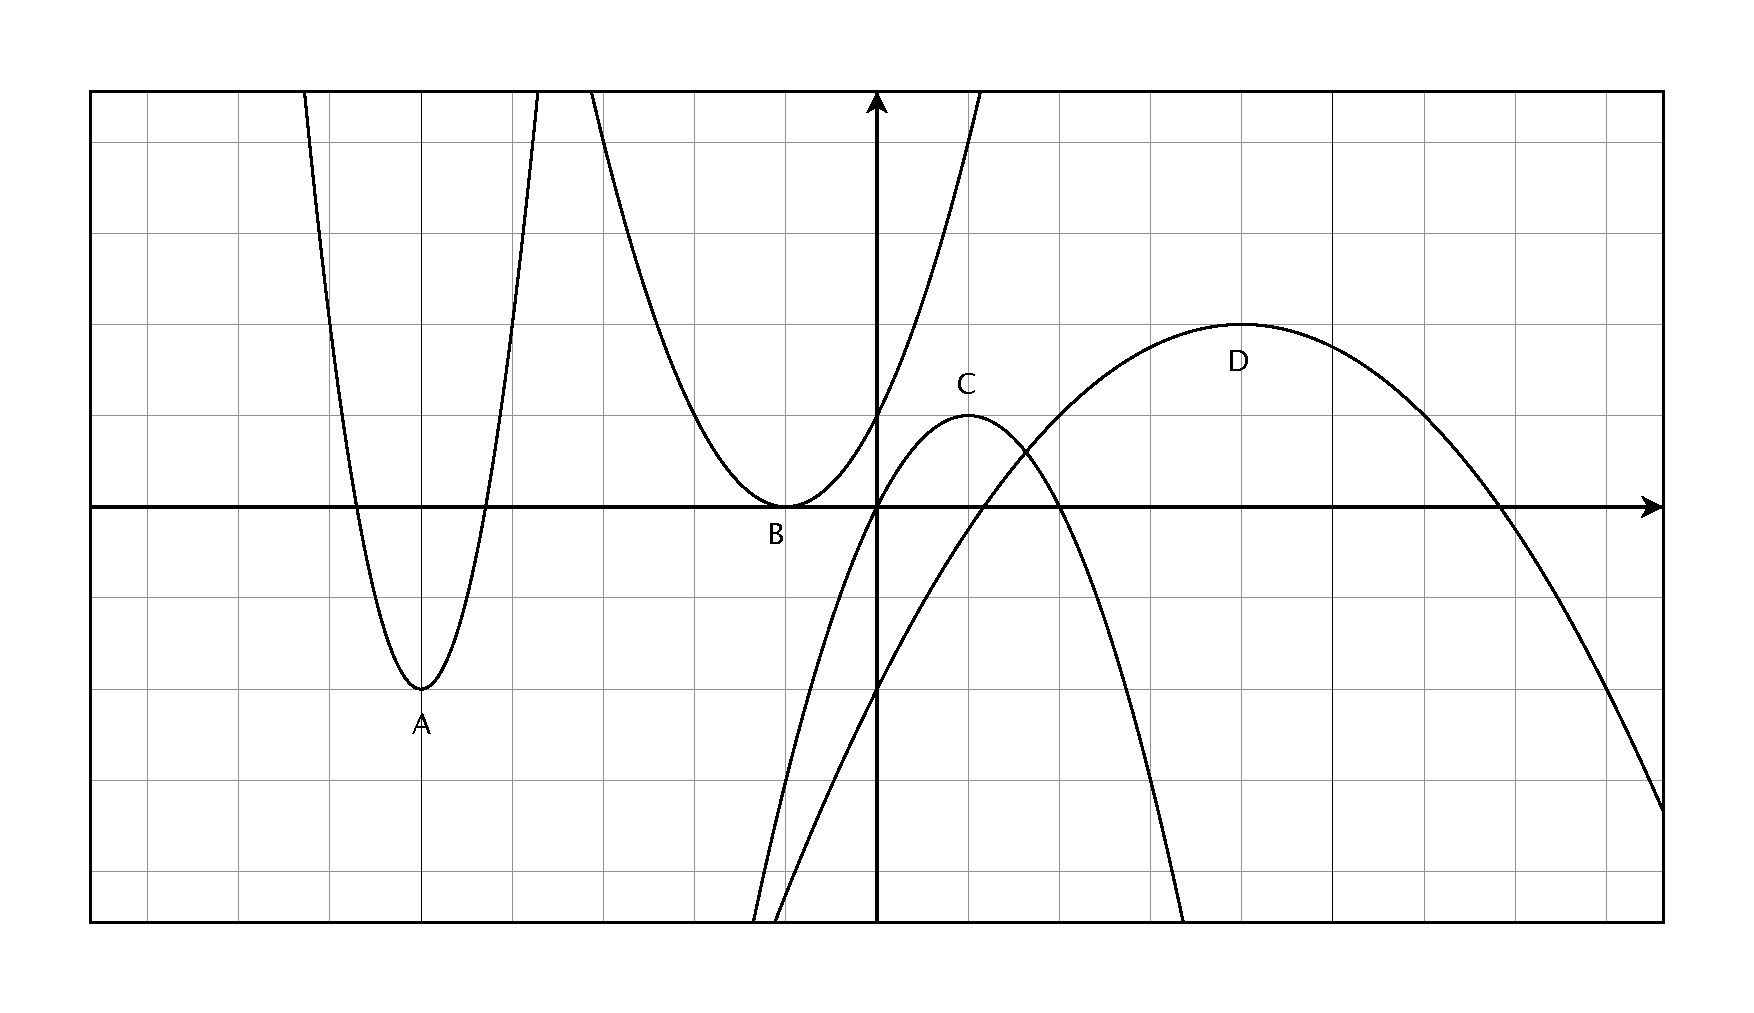
\includegraphics[scale=.3]{problem_7.eps}
%   \caption*{Problem 7}
% \end{figure}

% \begin{tabular}{cc}
% \toprule
% period & amplitude \\
% \midrule
%   $\pi$ & $2$ \\
% \bottomrule
% \end{tabular}

\title{Math 141 Notes \\ Section 2.8}
\date{February 20, 2013}

\begin{document}

\maketitle
\tableofcontents

\section{Homework 4 Notes}
\begin{itemize}
  \item You can read the vertex from the equation in standard form.  You don't have to use $x = \frac{-b}{2a}$ to
    find the vertex.

  \item Review completing the square.

  \item You don't have to complete the square to find the min/max.  You can just use $x_{min/max} = \frac{-b}{2a}$.  

  \item The domain of any polynomial is $(-\infty, \infty)$.  To find the range, find the min or max (depending on the
    sign of the $x^2$ coefficient).

  \item Explain grading scheme.

  \item use \verb+[] or ()+ instead of \verb+{}+ for ranges

  \item Include work.

  \item do in class:
    \begin{itemize*}
      \item section 2.5, problems 10 (no x-intercept) and 60
      \item section 2.6, problems 12, 13, 17, 29
    \end{itemize*}
    
\end{itemize}

\section{Proof of the Day}
\[
  \sum_{i = 1}^n = \frac{n(n + 1)}{2}
\]

\section{Function Composition Applications}
\begin{enumerate}
  \item Sand is pored into a conical pile whose radius and height are always equal, although both increase with time.
    The height of the pile $\unit[t]{seconds}$ after pouring begins is given by $h(t) = \unit[10 + 0.25t]{ft}$.  Express the
    volume of the pile as a function of $t$.

    The volume of a cone is $v = \frac{1}{3} \pi r^2 h$.

    \begin{solution}
      \begin{align*}
         v &= \frac{1}{3} \pi h^3 \\
       &= \frac{1}{3} (10 + 0.25t)^3 \\
      \end{align*}
    \end{solution}

  \item Tax Rates
    Alice has a mortgage and 401(k) plan.  She is in the 30\% tax bracket and pays 6\% Social Security tax on the first
    \$100,000 of her income, which is more than \$100,000.  She also spends 20\% of her income on taxable items which
    are taxed by the WA state sales tax of 10\%.

    Bob rents, is in the 25\% tax bracket and doesn't have a 401(k) plan.  He makes less than \$100,000 and spends 50\%
    of his income on taxable items.

    Find functions for each person's tax rate.  If Alice makes \$150,000 and Bob makes \$50,000, find their tax rates.

    \begin{solution}
      \begin{itemize}
        \item Alice's taxable income is: $A(x) = x - 15000 - 15000$
        \item Alice's tax, as a function of income is: $T(i) = 0.3i + 0.02i + 6000 = 0.32i + 6000$
        \item Alice's tax rate is $R \circ T \circ A$.
        \item Bob's taxable income is: $B(x) = x$
        \item Bob's tax rate is: $T(i) = 0.25i + 0.05i + 0.06i = 0.36i$
      \end{itemize}

      \begin{itemize*}
        \item Alice's effective tax rate is 30\%.
        \item Bob's effective tax rate is 36\%.
      \end{itemize*}
    \end{solution}
    
  \item A spherical balloon is inflated so that its radius at the end of $\unit[t]{seconds}$ is 
    \[
      r(t) = \unit[3 \sqrt{t} + 5]{cm}
    \]

    Express the volume and the surface area as functions of time.

    \begin{solution}
      \begin{align*}
        V(t) &= \frac{4}{3} \pi r^3 \\
        A(t) &= 4 \pi r^2 \\
      \end{align*}
    \end{solution}

\end{enumerate}

\section{One-to-One Functions}

Definition:
\begin{itemize*}
  \item draw domain/range picture for $x^2$ and $x^3$
  \item Every value for $f$ is unique: $x_1 \neq x_2 \Leftrightarrow f(x_1) \neq f(x_2)$
  \item horizontal line test.
\end{itemize*}

Examples:
\begin{itemize*}
  \item $f(x) = x^2$ is not one-to-one because, for example $f(-1) = f(1)$.
  \item $f(x) = x^3$ is one-to-one.
  \item $f(x) = \sqrt{x}$ is one-to-one.
  \item $f(x) = 2x - 3$ is one-to-one.
  \item $f(x) = 2$ is not one to one.
  \item $f(x) = |x|$ is one-to-one.
\end{itemize*}

\section{Inverse Functions}
\subsection{Definition}
\begin{itemize}
  \item Inverse function undoes effect of original function: $f(f^{-1}(x)) = f^{-1}(f(x)) = x$
  \item examples plus/minus, multiple/divide, cube/cube root 
\end{itemize}

\subsection{Finding Inverse Functions Algebraically}
\begin{itemize*}
  \item write function as $y = \text{expression}$
  \item solve for $x$ in terms of $y$
  \item exchange $x$ and $y$ in the result so the final function is a function of $x$.
  \item verify by checking to see that $f(f^{-1}(x) = f^{-1}(f(x)) = x$.
\end{itemize*}

\subsection{Examples}
\begin{itemize}
  \item $f(x) = x + 2$, $f^{-1}(x) = x - 2$
    
  \item $f(x) = 2x + 1$, $f^{-1(x)} = \frac{x - 1}{2}$  
    
  \item $f(x) = \frac{1}{x - 1}$, $f^{-1}(x) = \frac{x + 1}{x}$

  \item $f(x) = \frac{x - 1}{x + 5}$, $f^{-1}(x) = \frac{5y + 1}{1 - y}$

  \item $f(x) = x^3 + 1$, $f^{-1}(x) = \sqrt[3]{x - 1}$

  \item with restricted domain: $f(x) = x^2 + 1$, $x \geq 0$; $f^{-1}(x) = \sqrt[2]{x - 1}$, $x \geq 1$

\end{itemize}

\subsection{Finding Inverse Functions Graphically}

$f^{-1}(x)$ is the reflection of $f(x)$ around the line $y = x$.

\subsection{Applications}

\begin{enumerate}
  \item Hourly wage is \$8.00 per hour plus \$0.75 per unit produced.  Hourly wage in terms of number of items is:
    \[
      w(n) = 8 + 0.75n
    \]

    \begin{enumerate}[a]
      \item Find the inverse function.  
        \begin{solution}
          \[
            f^{-1}(w) = n(w) = \frac{4w - 32}{3}
          \]
        \end{solution}

      \item What does the inverse function represent? 
        \begin{solution}
          It's the number of items made each hour by someone with an hourly wage of $w$.
        \end{solution}

      \item Find the number of units produced hourly by someone with a wage of \$22.25.
        \begin{solution}
          \[
            n(22.25) = 19
          \]
          As a check, the wage for someone who makes 19 units per hour would be:
          \[
            w(19) = 22.25
          \]
        \end{solution}
    \end{enumerate}

  \item You need 50 pounds of two items which cost \$1.25 and \$1.60 per pound.  The total cost is:
    \[
      C(n) = 1.25n + 1.60(50 - n) = 80 - 0.35n
    \]
    where $n$ is the number of pounds of the cheaper item.

    \begin{enumerate}[a]
      \item Find the inverse function.  What does it represent?
        \begin{solution}
          \[
            N(c) = 229 - 2.86c
          \]
          This is the number of pounds of the cheaper item you will end up with if you spend $c$ dollars.
        \end{solution}
        
      \item What is the domain of the inverse function?
        \begin{solution}
          You have to get between 0 and 50 pounds of the cheaper item.  
          \begin{itemize*}
            \item If you get 0 pounds of the cheap one, you have to spend $1.60 \cdot 50 = \$80$.
            \item If you get 50 pounds of the cheap one, you spend $1.25 \cdot 50 = 62.50$.
          \end{itemize*}

          So the domain of the inverse function is: $[62.5, 80]$. 
        \end{solution}

      \item How much of the cheap item to you get by spending \$70?
        \begin{solution}
          \[
            N(70) \approx \unit[28.8]{pounds}
          \]
        \end{solution}
    \end{enumerate}
\end{enumerate}

\section{Miscellaneous}

Talk to Jeff Grote about 
\begin{itemize*}
  \item piecewise defined functions
  \item sign charts
\end{itemize*}

\end{document}
